% GENERATED by scripts/make_figure_pages.py from captions/ and figures/.
% Do not edit by hand.

\begin{figure}[p]
\centering
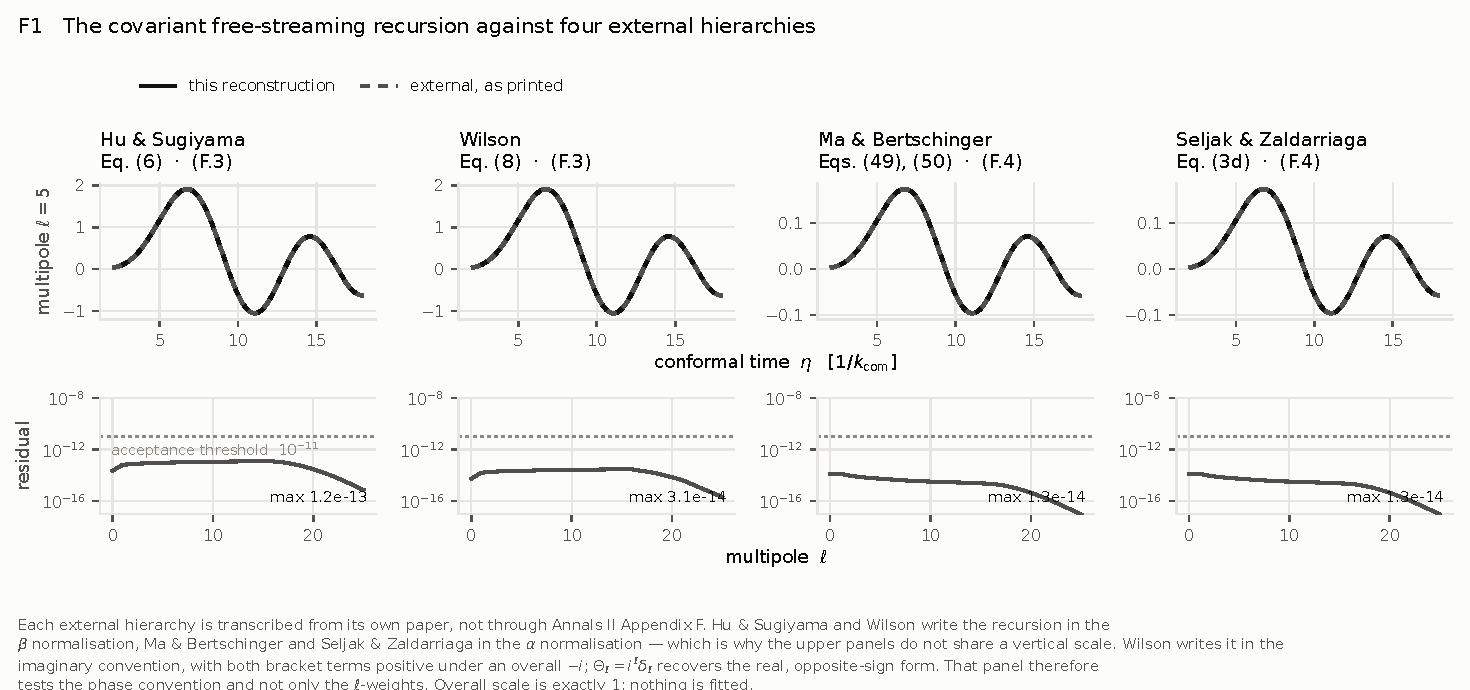
\includegraphics[width=\textwidth]{figures/f1-appendix-f-v1.0.0.pdf}
\caption[The covariant free-streaming recursion against four external hierarchies]{\textbf{F1 --- The covariant free-streaming recursion against four external hierarchies.} The covariant free-streaming recursion of \emph{Annals~II} Appendix~F, integrated from a unit monopole, against four external treatments of the same hierarchy. Each is transcribed from its own paper, never through Appendix~F. \textbf{Upper panels, context:} the reconstruction and the external form at $\ell=5$; they coincide. The panels do \emph{not} share a vertical scale, because two normalisations are on display. \textbf{Lower panels, the claim:} $\max_\eta|\mathrm{external}-\mathrm{reconstruction}|$ against $\ell$, with the acceptance threshold marked. Hu \& Sugiyama write the recursion in the $\beta$ normalisation and Ma \& Bertschinger and Seljak \& Zaldarriaga in the $\alpha$ normalisation, which is why Appendix~F prints both (F.3) and (F.4); a basis phase leaking into the couplings would break at least one match. Overall scale is exactly $1.000000000$ --- nothing is fitted. Four panels from five sources: Wilson \& Silk (1981) is the earliest, but at $K=0$ it is Wilson (1983) Eq.~(8) exactly, so it is credited rather than drawn.\\[2pt]\footnotesize\emph{Evidence category:} cross-check. \emph{Generated by} \texttt{scripts/figure\_f1\_appendix\_f.py}. \emph{Standalone caption:} \texttt{captions/F1-appendix-f.md}.}
\label{fig:f1}
\end{figure}

\begin{figure}[p]
\centering
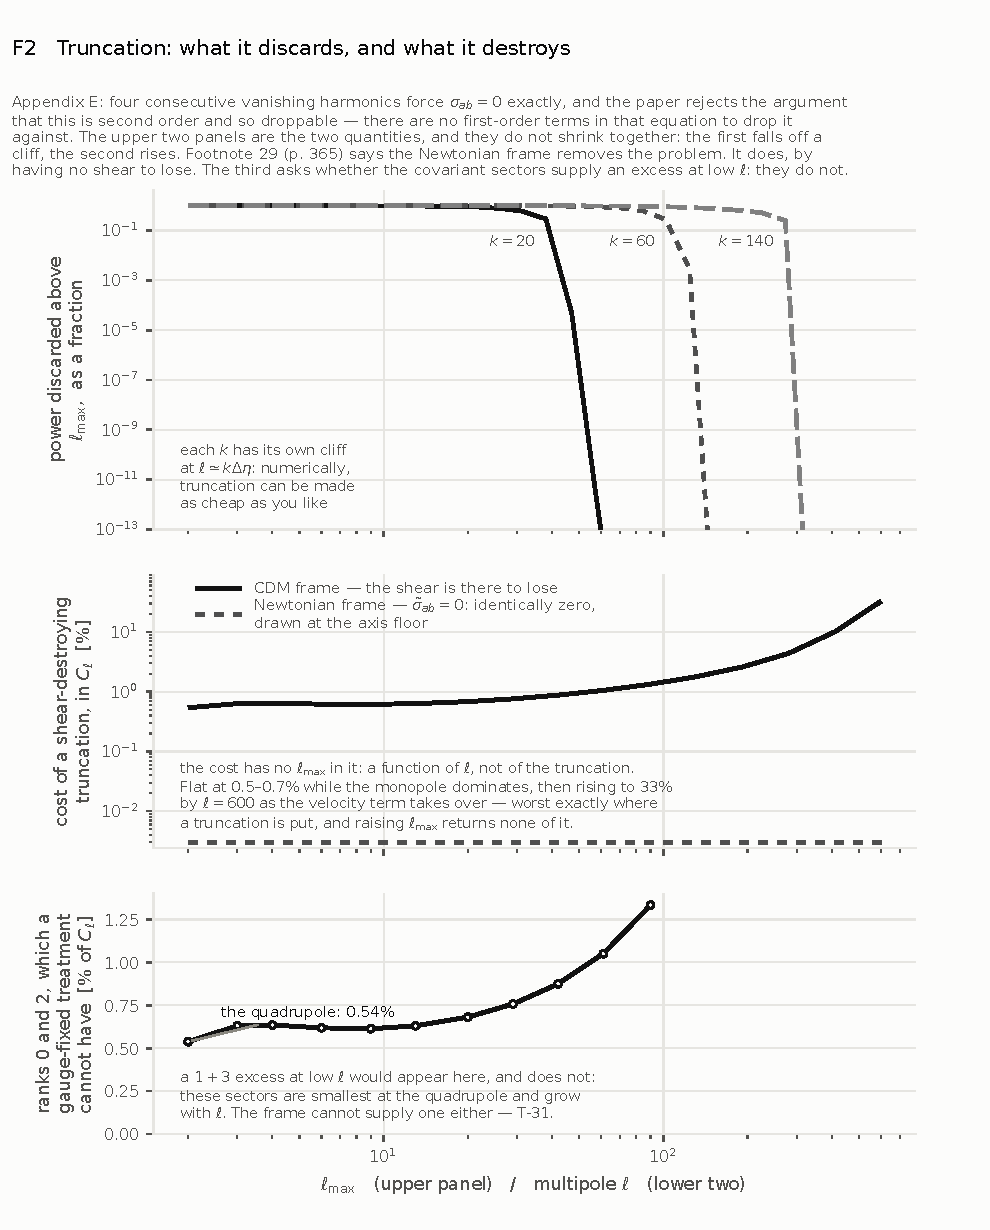
\includegraphics[width=\textwidth]{figures/f2-truncation-v1.2.0.pdf}
\caption[What a truncation discards, and what it destroys]{\textbf{F2 --- What a truncation discards, and what it destroys.} Appendix~E of \emph{Annals~II} proves that four consecutive vanishing harmonics force $\sigma_{ab}=0$ exactly. This figure makes that quantitative in both frames, and the two panels answer two different questions that a single ``truncation error'' would blur.\\[2pt] \textbf{What a truncation \emph{discards}} falls off a per-$k$ cliff at $\ell\simeq k\,\Delta\eta$: above the cliff there is nothing left to keep, and the tail above $\ell=600$ is identically zero at every probe mode. \textbf{What it \emph{destroys}} has no $\ell_{\max}$ in it at all. Setting $\sigma_{ab}\to0$ costs $0.54$--$0.68\%$ out to $\ell\simeq20$, rises monotonically above $\ell=20$, and reaches $32.6\%$ by $\ell=600$ \textbf{[pre-T-57 values; this figure is superseded --- see the dagger]} --- a cost that grows with the multipole rather than being bounded by it, which is why a truncation argument cannot retire the shear.\\[2pt] \textbf{Footnote~29 (p.~365) is checked and upheld.} In the Newtonian frame the cost is \emph{identically zero}, median and maximum alike, because that frame has no shear to lose --- which is the content of the footnote's claim that the Newtonian specialisation removes the truncation problem. The script raises rather than draws if the Newtonian rank-0/2 sectors are ever non-empty, so the claim is a gate and not a caption.\\[2pt] \textbf{The third panel is the one that reports a negative result.} The rank-0/2 share is flat at the quadrupole ($0.54\%$) and rises only with $\ell$: a $1+3$ excess at low $\ell$ would appear here, and does not. That question is parked as \textbf{Q5}, and this panel is what parks it honestly.\\[2pt]$^{\dagger}$\,\emph{Superseded by finding} \textbf{T-57}\emph{; see} \texttt{provenance/BUNDLE-DEFECTS-v1.md}. \textbf{Its $k$ grid runs to 1900, not 420} --- finding \textbf{T-32}, where every v1.2.0 figure had been drawn on a grid stopping at the peak of the shear integrand. At $k_{\max}=1900$ against $k_D=754.6$ the damping envelope is $1.8\times10^{-3}$, and dropping the grid's top decile moves the cost by $3.4\times10^{-9}$. The lesson recorded there is the rule here: vary the limit and the resolution separately, because one grid number conflates them.\\[2pt]\footnotesize\emph{Evidence category:} cross-check. \emph{Generated by} \texttt{scripts/figure\_f2\_truncation.py}. \emph{Standalone caption:} \texttt{captions/F2-truncation.md}.}
\label{fig:f2}
\end{figure}

\begin{figure}[p]
\centering
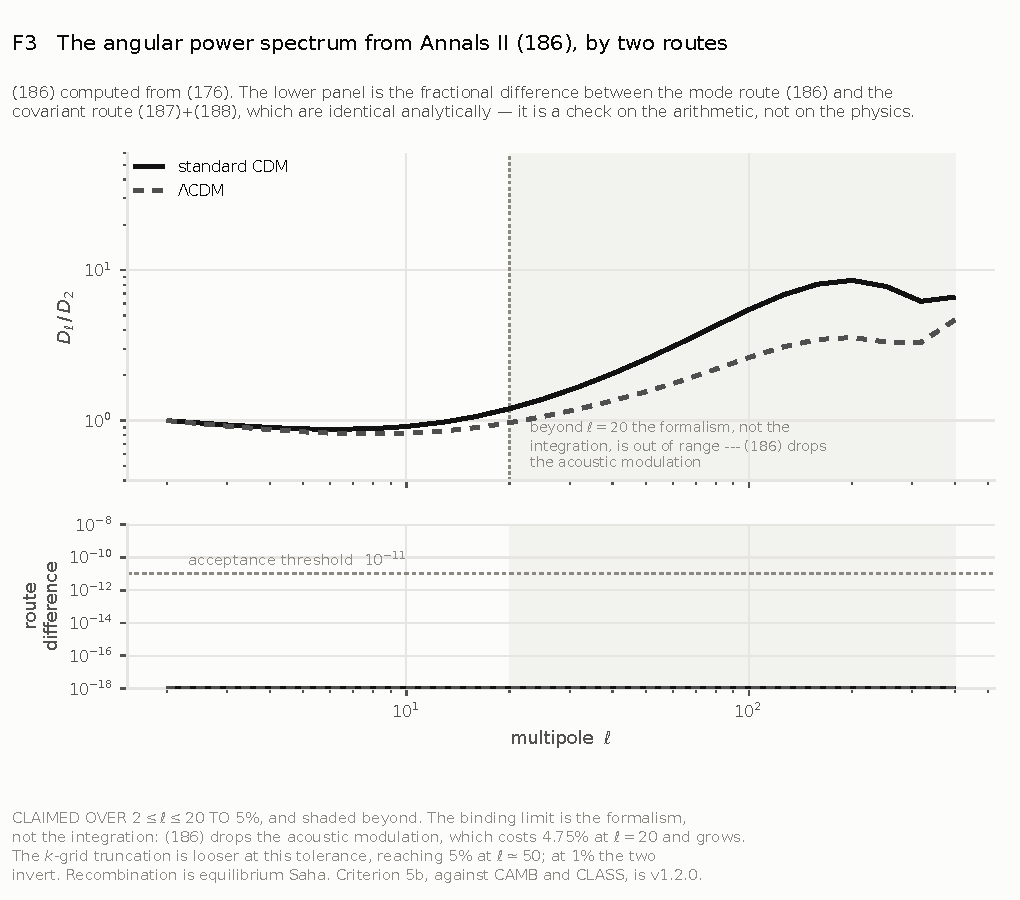
\includegraphics[width=\textwidth]{figures/f3-angular-spectrum-v1.0.0.pdf}
\caption[The angular power spectrum from Annals II (186), by two routes]{\textbf{F3 --- The angular power spectrum from Annals II (186), by two routes.} Eq.~(186) computed from Eq.~(176), for the standard-CDM model of \S8.3.2 and for $\Lambda$CDM, which \emph{Annals~II} does not treat. \textbf{Upper panel:} $D_\ell=\ell(\ell+1)C_\ell/2\pi$, each normalised to its own $\ell=2$ value, so that the comparison is of \emph{shape} and not of an amplitude neither model fixes here. \textbf{Lower panel:} the fractional difference between the mode route of (186) and the covariant route of (187) with (188). Those two are identical analytically, so the panel is a check on the arithmetic and not on the physics --- and it is worth having, because it caught a factor of four in this bundle's own harmonic weights before any figure was drawn. It sits at $10^{-16}$, five orders below the $10^{-11}$ acceptance threshold.\\[2pt]\footnotesize\emph{Evidence category:} recovery. \emph{Generated by} \texttt{scripts/figure\_f3\_angular\_spectrum.py}. \emph{Standalone caption:} \texttt{captions/F3-angular-spectrum.md}.}
\label{fig:f3}
\end{figure}

\begin{figure}[p]
\centering
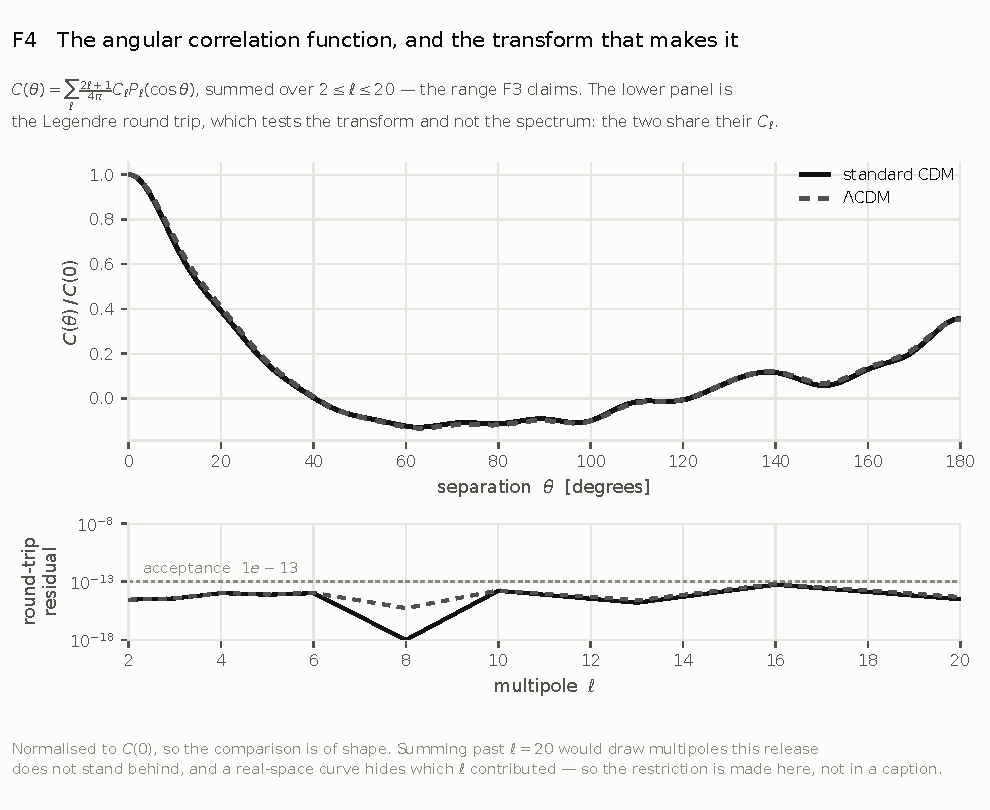
\includegraphics[width=\textwidth]{figures/f4-correlation-v1.0.0.pdf}
\caption[The angular correlation function, and the transform that makes it]{\textbf{F4 --- The angular correlation function, and the transform that makes it.} $C(\theta)=\sum_\ell\frac{2\ell+1}{4\pi}C_\ell P_\ell(\cos\theta)$, the real-space view of Figure~3: the same content read as a correlation between two directions separated by $\theta$ rather than as power at a multipole. \textbf{Upper panel:} $C(\theta)/C(0)$ for standard CDM and $\Lambda$CDM, summed over $2\le\ell\le20$ --- the range Figure~3 claims, bounded by (186) dropping the acoustic modulation. Summing further would draw multipoles this release does not stand behind, and a real-space curve hides which $\ell$ contributed, so the restriction is made in the transform rather than in this caption. \textbf{Lower panel:} the Legendre round trip $C_\ell\to C(\theta)\to C_\ell$, at $4\times10^{-14}$ and $7\times10^{-14}$ against an acceptance of $10^{-13}$. It tests the transform and \emph{not} the spectrum --- the two share their $C_\ell$ --- which is the same caution Figure~3's residual panel carries and for the same reason.\\[2pt]\footnotesize\emph{Evidence category:} acceptance. \emph{Generated by} \texttt{scripts/figure\_f4\_correlation.py}. \emph{Standalone caption:} \texttt{captions/F4-correlation.md}.}
\label{fig:f4}
\end{figure}

\begin{figure}[p]
\centering
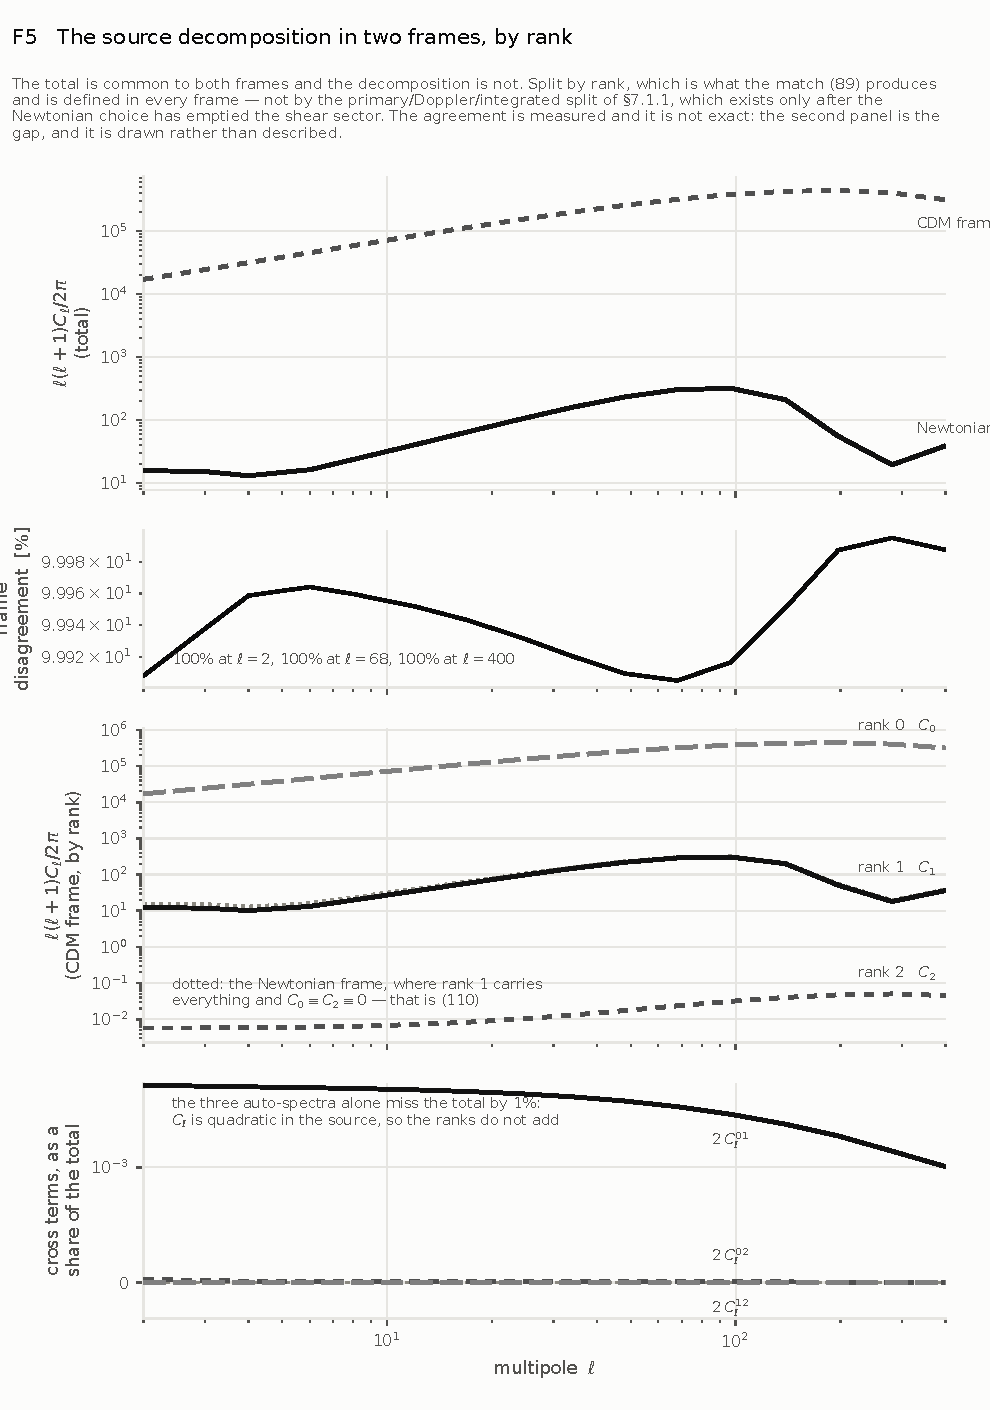
\includegraphics[width=\textwidth]{figures/f5-sources-v1.2.0.pdf}
\caption[The source decomposition, by rank, in two frames]{\textbf{F5 --- The source decomposition, by rank, in two frames.} The integral solution~(102) carries three coefficients $C_0$, $C_1$, $C_2$ --- one per PSTF rank --- and this figure draws them, in the Newtonian frame and in the CDM frame, against $\ell$.\\[2pt] \textbf{Drawn in ranks, not in the Newtonian three-way split of \S7.1.1.} That was the PI's call, 2026-10-14, and it is a scientific choice rather than a presentational one: the primary/Doppler/integrated split is \emph{defined only in the frame it is written in}, while the rank decomposition is what~(89) produces and is defined in every frame. A figure comparing two frames must be drawn in a decomposition both of them have.\\[2pt] \textbf{The ranks sum to the total}, to $0$ exactly in the Newtonian frame and $4.1\times10^{-16}$ in the CDM frame --- which is the check that the decomposition is a decomposition and not three curves that happen to be near the answer. At the $C_\ell$ level the autos and twice the crosses reproduce $C_\ell$ to $4.7\times10^{-16}$ while the autos \emph{alone} are off by $0.10$: $C_\ell$ is quadratic in the transfer, so the cross terms are not a correction to be neglected but half the statement.\\[2pt] \textbf{The frame disagreement is the result, and it is its own panel.} The two frames' $C_\ell$ differ by a median of $15\%$ over $2\le\ell\le400$, worst $49\%$ \textbf{[pre-T-57/T-59 values; this figure is superseded --- see the dagger]}. That is not a defect: $C_\ell$ as computed here is built from frame-dependent pieces, and the invariance statement~(102) satisfies is about the \emph{total} at fixed $k$, which diagnostic~D6 measures separately. The median moved from $11\%$ to $15\%$ when finding \textbf{T-37} wired the transfer function, which is the kind of movement a figure should report rather than absorb.\\[2pt]$^{\dagger}$\,\emph{Superseded by findings} \textbf{T-57}\emph{,} \textbf{T-59}\emph{; see} \texttt{provenance/BUNDLE-DEFECTS-v1.md}.\\[2pt]\footnotesize\emph{Evidence category:} cross-check. \emph{Generated by} \texttt{scripts/figure\_f5\_sources.py}. \emph{Standalone caption:} \texttt{captions/F5-sources.md}.}
\label{fig:f5}
\end{figure}

\begin{figure}[p]
\centering
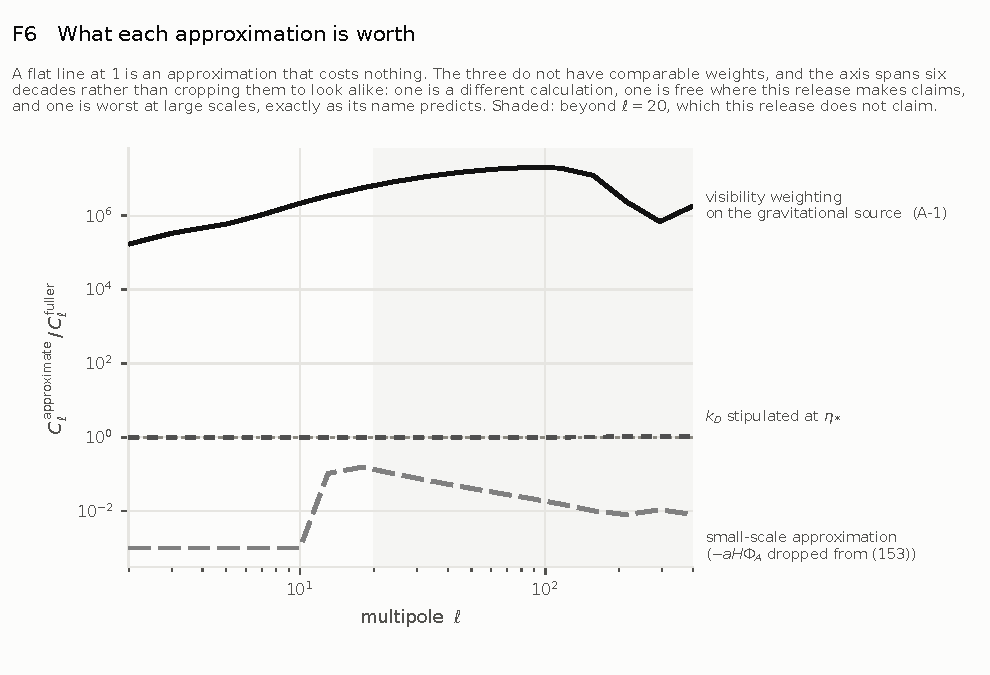
\includegraphics[width=\textwidth]{figures/f6-approximations-v1.1.0.pdf}
\caption[What each approximation is worth]{\textbf{F6 --- What each approximation is worth.} Each series is $C_\ell^{\mathrm{approximate}}/C_\ell^{\mathrm{fuller}}$ for standard CDM, so the panel is scale-free and a flat line at unity is an approximation that costs nothing. \emph{Annals~II} makes three narrowing choices which this bundle reproduces rather than corrects, because reproducing a paper means reproducing its approximations (decision~S15); they are recorded as \textbf{A-n} in \texttt{provenance/SOURCE-APPROXIMATIONS-v1.md}, deliberately apart from the defects recorded as \textbf{B-n}. This is the one place their cost is a number rather than an adjective.\\[2pt] \textbf{The three do not have comparable weights, and that is the result}, so the axis spans six decades rather than cropping them to look alike. The visibility weighting on the gravitational source (A-1) runs to $10^4$--$10^6$: it is a \emph{different calculation}, not a perturbation of one, which is why \texttt{Weighting} has no default. Stipulating $k_D$ at last scattering costs under $0.1\%$ across the claimed range and about $5\%$ by $\ell=400$ --- it \textbf{vindicates the release}, which takes the cheap choice where it makes claims. The small-scale approximation, dropping $-aH\Phi_A$ from~(153) and so producing the printed oscillator~(154), departs from unity most at \emph{large} scales, which is what its name predicts. \\[2pt] \textbf{A correction kept because it nearly became this figure.} The $k_D$ series was first computed with $k_D(\eta)$ along the whole ray. After last scattering $\kappa'\to0$, so $1/\kappa'$ in (dif-damp) diverges and $k_D$ collapses, damping every integrated source to nothing --- a plasma formula evaluated in a universe that no longer has a plasma. That version reported the release's choice as costing a factor of nine at $\ell=2$; the factor was the artefact. Clamped to $k_D(\min(\eta,\eta_*))$ the comparison is a real one. Shaded: beyond $\ell=20$, which this release does not claim.\\[2pt]\footnotesize\emph{Evidence category:} diagnostic. \emph{Generated by} \texttt{scripts/figure\_f6\_approximations.py}. \emph{Standalone caption:} \texttt{captions/F6-approximations.md}.}
\label{fig:f6}
\end{figure}

\begin{figure}[p]
\centering
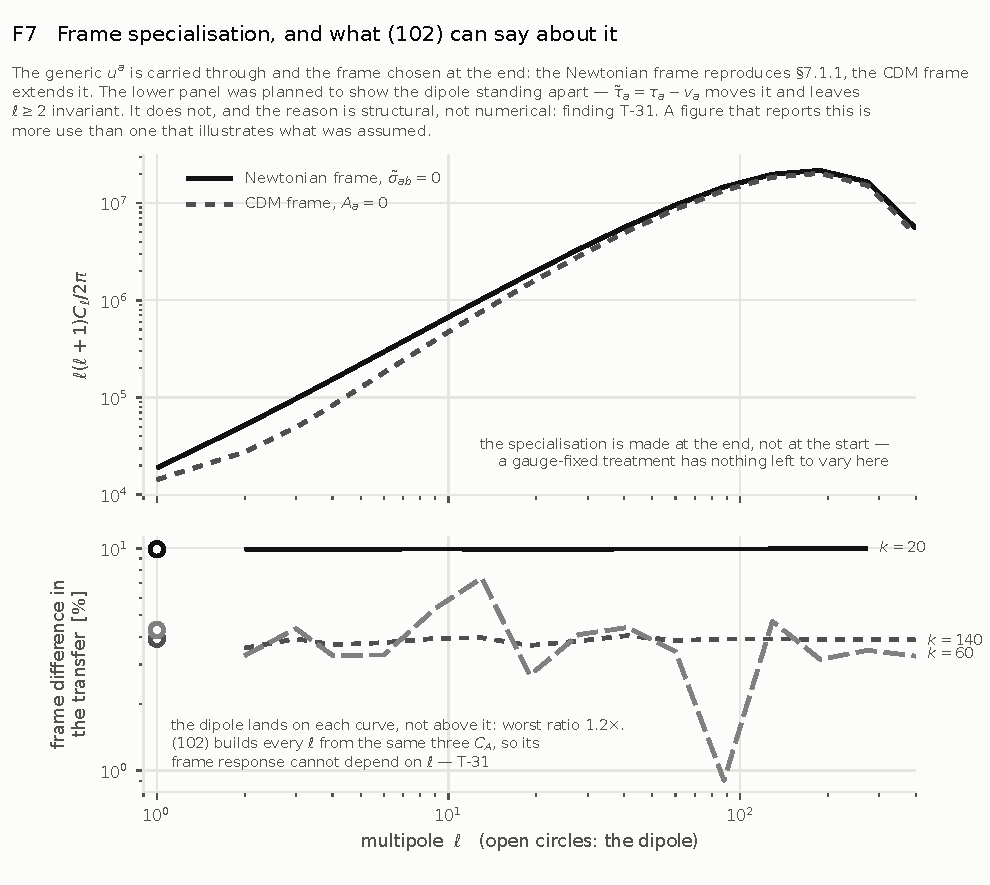
\includegraphics[width=\textwidth]{figures/f7-frames-v1.2.0.pdf}
\caption[Frame specialisation, and a planned claim that was false]{\textbf{F7 --- Frame specialisation, and a planned claim that was false.} \textbf{This figure reports that its own planned claim is false, and that is why it is here.} It was designed to show the dipole standing an order of magnitude apart from the higher multipoles under a change of frame --- the dipole being the one multipole a boost moves at first order. It does not. The dipole lands on each curve instead: worst ratio $1.25\times$ over the probe set, and $1.00\times$ at $k=20$.\\[2pt] \textbf{The reason is structural and is finding T-31.} Equation~(102) builds \emph{every} $\ell$ from the same three coefficients $C_A$, so a frame change that moves $C_1$ moves every multipole built on it in the same proportion. A frame response that depended on $\ell$ would contradict the equation's own form, and \texttt{test\_102\_cannot\_make\_its\_frame\_response\_depend\_on\_the\_multipole} asserts that it does not. The spread \emph{over} $\ell$ does grow with $k$ --- $1.01$, $1.14$, $8.14$ at $k=20$, $60$, $140$ --- but that is the transfer function's $k$ dependence, not the frame's $\ell$ dependence.\\[2pt] \textbf{A figure that had been drawn to its plan would have been drawn wrong.} The plan is kept in \texttt{captions/FIGURE-PLAN-v1.0.0.md} and the outcome is kept here, because a reproduction bundle whose figures only ever confirm their captions is not measuring anything.\\[2pt] \textbf{Its environment is built for the $k$ grid, not for the probe modes} --- finding \textbf{T-34}, where this figure sized its $\eta$ grid for $k=140$ and then integrated to $k=420$. \texttt{check\_k} now raises rather than interpolating past what the grid resolves.\\[2pt]\footnotesize\emph{Evidence category:} diagnostic. \emph{Generated by} \texttt{scripts/figure\_f7\_frames.py}. \emph{Standalone caption:} \texttt{captions/F7-frames.md}.}
\label{fig:f7}
\end{figure}

\begin{figure}[p]
\centering
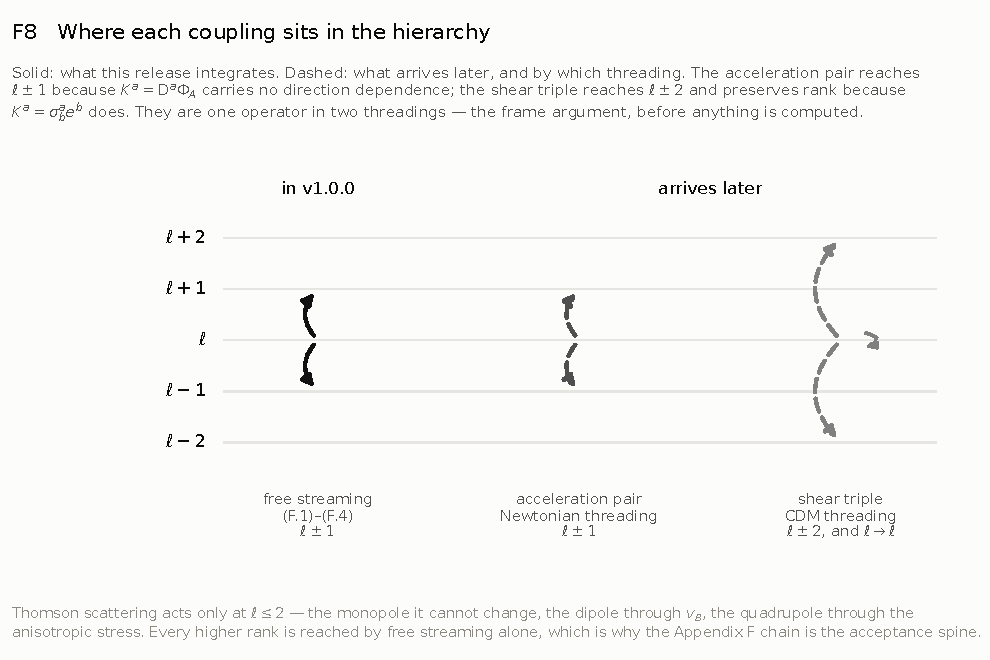
\includegraphics[width=\textwidth]{figures/f8-schematic-v1.1.0.pdf}
\caption[Where each coupling sits in the hierarchy]{\textbf{F8 --- Where each coupling sits in the hierarchy.} The one released figure that computes nothing: a statement about the \emph{structure} of the exact divergence hierarchy, read off the equations rather than measured. It is generated by a script like every other figure, so that the manifest covers it --- a hand-drawn diagram is the one artefact that can drift without any gate noticing.\\[2pt] \textbf{Solid:} what this release integrates. Free streaming, (F.1)--(F.4), couples rank $\ell$ to $\ell\pm1$ and to nothing else, which is the whole of v1.0.0's hierarchy and the reason the Appendix~F chain is the acceptance spine. \textbf{Dashed:} what arrives later, and by which frame. The acceleration pair reaches $\ell\pm1$ because $K^a=\mathrm{D}^a\Phi_A$ carries no direction dependence of its own; the shear triple reaches $\ell\pm2$ \emph{and} preserves rank because $K^a=\sigma^a{}_be^b$ does. The rank-preserving coupling exists only when $K^a$ depends on direction, and is the single structural difference between the two frames.\\[2pt] Both are the same operator $K_\perp^a\partial/\partial e^a$, and the number of ranks each reaches is fixed by that one property. \textbf{That is the whole content of the frame argument, visible before any of it is computed.} Decision S9 is drawn as well as asserted: every coupling in the solid half is a ratio of linear polynomials and tends to a constant, so an $O(\ell)$ coupling wired in early would fail \texttt{tests/test\_appendix\_f\_chain.py} at large $\ell$.\\[2pt]\footnotesize\emph{Evidence category:} schematic. \emph{Generated by} \texttt{scripts/figure\_f8\_schematic.py}. \emph{Standalone caption:} \texttt{captions/F8-schematic.md}.}
\label{fig:f8}
\end{figure}

\begin{figure}[p]
\centering
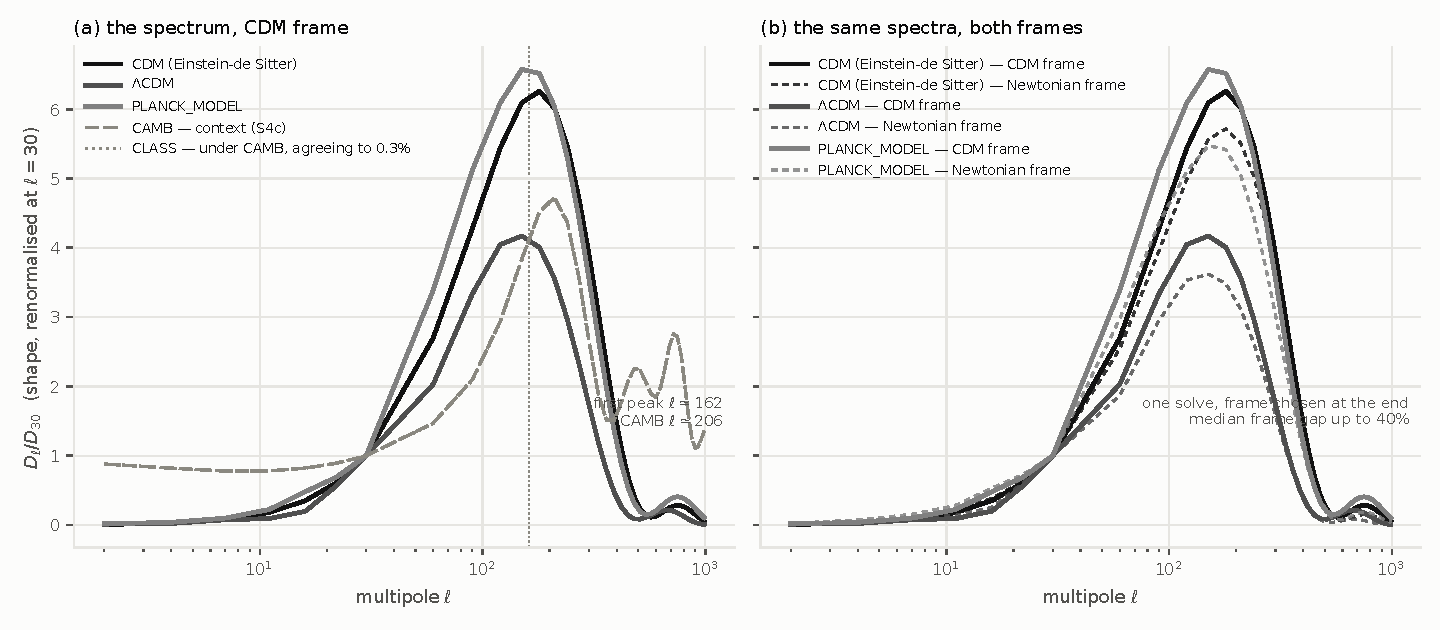
\includegraphics[width=\textwidth]{figures/f9-acoustic-spectrum-v1.2.0.pdf}
\caption[The angular spectrum with the acoustic peaks, in both frames]{\textbf{F9 --- The angular spectrum with the acoustic peaks, in both frames.} \textbf{The release's deliverable} (decision~S1): the angular power spectrum for the three backgrounds this bundle ships --- CDM (Einstein--de Sitter), $\Lambda$CDM, and the stamped Planck~2018 set with a photon-only radiation era whose $\Omega_\gamma h^2$ is \emph{derived} from $T_{\rm CMB}$. Shape, $D_\ell$ renormalised at $\ell=30$, because neither this bundle nor the external codes fixes $A_s$ the same way and an amplitude comparison would measure a normalisation.\\[2pt] \textbf{Panel (a) --- the spectrum.} The peaks and the damping tail come from \emph{Annals~II}'s own equations: the integral solution~(102) with the Bond--Efstathiou transfer function driving the oscillation per mode, and the diffusion scale from \textbf{(dif-damp-correct)} at $f_2=3/4$, which is the antecedent's own corrected coefficient rather than a departure from it (\textbf{T-43}). \textbf{This shows that} the almost-Friedmann--Lemaitre formulation, carried to the damping scale, produces acoustic structure without anything being imported from a Boltzmann code.\\[2pt] \textbf{CAMB and CLASS are drawn as context and are not a target} --- decision~\textbf{S4c}. Criterion~5b is gated on this bundle's own pipeline, (102) against (177)--(179), at $9.5\times10^{-6}$ against $10^{-3}$. The distance to the external codes is large, expected, and \emph{itemised rather than totalled} in \texttt{provenance/CRITERION-5B-v1.md}: $97.8\%$ across the plateau, $137\%$ across the peaks, of which the damping coefficient alone is $17.2\%$. The first peak is quoted from a \emph{parabolic interpolation} through the grid maximum and its neighbours, because the $\ell$ grid steps by 30 across the acoustic band and reading the peak off it directly would assert a precision the sampling does not have.\\[2pt] \textbf{Panel (b) --- the panel a gauge-fixed treatment cannot draw.} The same spectra in \emph{both} frames, from \emph{one} solve: \texttt{coefficient\_sets} returns the Newtonian and CDM triples together, because~(102) is carried with a generic $u^a$ and the frame is chosen at the end. \textbf{This shows that} the frame is a choice made after the derivation rather than an assumption built into its start --- the claim the $1+3$ covariant approach exists to make, drawn here rather than asserted. The median frame gap reaches $40\%$. \textbf{This caption read ``which is a result and not a defect''; that reading is superseded by T-59 and T-74 and is withdrawn.} The gap is now understood as the third symptom of one term --- the bare $\kappa'$ carried inside $C_1$, \textbf{T-101} and \textbf{T-121} --- and not as a property of the formulation. What remains true of the original reading is only this: $C_\ell$ is quadratic in frame-dependent pieces, while the invariance~(102) satisfies is a statement about the total at fixed $k$, measured separately by~D6.\\[2pt]$^{\dagger}$\,\emph{Superseded by findings} \textbf{T-59}\emph{,} \textbf{T-74}\emph{; see} \texttt{provenance/BUNDLE-DEFECTS-v1.md}.\\[2pt]\footnotesize\emph{Evidence category:} acceptance. \emph{Generated by} \texttt{scripts/figure\_f9\_acoustic\_spectrum.py}. \emph{Standalone caption:} \texttt{captions/F9-acoustic-spectrum.md}.}
\label{fig:f9}
\end{figure}
